\appendix
\section{Photos, thoughts and ideas}
\frame[noframenumbering]{
\begin{itemize}
	\iitem{W. Hirsch, S. Smale, \textit{"Introduction to Chaos"};}
	\iitem{"Chaos Through-Wall Imaging Radar" by Hang Xu et al. (2009)}
	\iitem{\textit{"Chaos-based communications"} by Apostolos Argyris et al. (2005);}
	\iitem{M. Pecora, L. Carroll, \textit{"Synchronization in Chaotic Systems"} (1990);}
	\iitem{\textit{"Physics and Applications of Laser Diode Chaos"} by
M. Sciamanna, and K. A. Shore (2015);}
	\iitem{\textit{"Chaotic Pulsing and Quasi-Periodic Route to
Chaos in a Semiconductor Laser with Delayed
Opto-Electronic Feedback"} by
S. Tang and J. M. Liu (2001)}
	\iitem{\textit{"Semiconductor Lasers I
Fundamentals"} Chapter I by Ch.I by Bin Zhao, Amnon Yariv (1998)}
\end{itemize} \frametitle{Literature}}
\frame[noframenumbering]{
\begin{figure}[h]
    \centering
    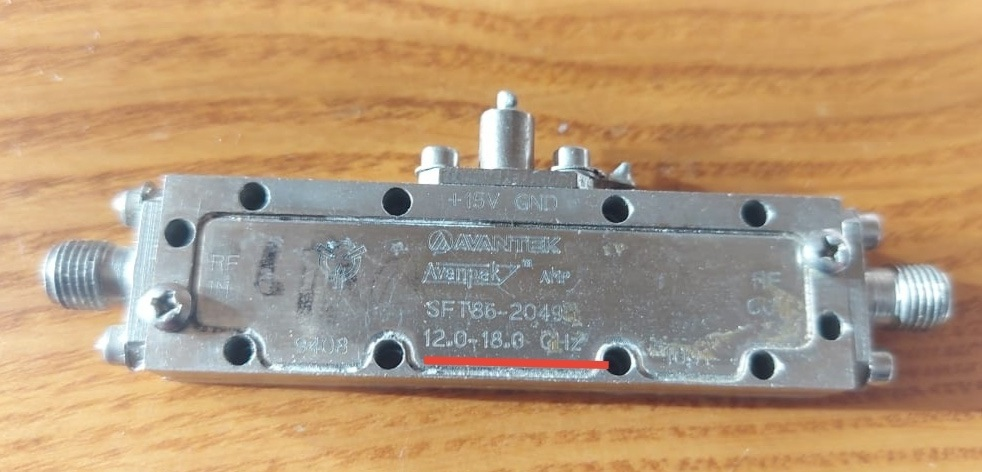
\includegraphics[width=0.8\textwidth]{images/newhope.jpg}
    \caption{Exactly from the article that we were inspired by...}
    %\label{fig:}
\end{figure}
 \frametitle{A new experimental set up came}}

\section{Theory expanded}

\frame[noframenumbering]{
To start the laser idea we need to obtain:
\begin{itemize}
	\iitem{Solution of the Schr\"odinger equation in a semiconductor medium for the wavefunction of an electron;}
	\iitem{Induced polarization for distribution of holes and electrons in a semiconductor;}
	\iitem{Interaction of electrons in a semiconductor with an wave equation and outer electric field.}
\end{itemize}
 \frametitle{The concept of a semiconductor laser}}

\frame[noframenumbering]{
We will need the Schr\"odinger equation:
\begin{equation*}
	H_{\text{crystal}} \Psi_n(\vc{r}) = \left[\frac{\vc{p}^2}{2 m_0} + U_p(\vc{r})\right] \Psi_n(\vc{r})
\end{equation*}
where $\vc{p} = - i \hbar \nabla$ is the momentum operator, $m_0$ is the free electron mass, $U_p(\vc{r})$ is th periodic potential of the bulk semiconductor.

The solution is the Bloch function:
\begin{equation*}
	\Psi_{n, \smallvc{k}}(\vc{r}) = u_{n, \smallvc{k}}(\vc{r}) \frac{1}{\sqrt{V}} e^{i \smallvc{k} \cdot \smallvc{r}}.
\end{equation*}
 \frametitle{Electronic states in a semiconductor}}

\frame[noframenumbering]{
In case of an optical field the Hamiltonian changes to
\begin{equation*}
	H = \frac{[\vc{p} + e \vc{A}(\vc{r}, t)]^2}{2 m_0} + U_p(\vc{r}) = H_\text{crystal} + H'
\end{equation*}
$\vc{A}(\vc{r},t)$ is the vector potential of the optical field. So the interaction Hamiltonian 
\begin{equation*}
	H' \approx \frac{e}{m_0} \vc{A}(\vc{r},t) \cdot \vc{p}.
\end{equation*} \frametitle{Hamilton in an outer field}}

\frame[noframenumbering]{
For y-propagating field: $E(\vc{r}, t) = \frac{1}{2} E_0 e^{i (\beta y - \omega t)} + \const$ the Hamiltonian is
\begin{equation*}
	H' = \frac{1}{2} \mu(k_q,x,z) [E_0 e^{i (\beta y - \omega t)} + \const]
\end{equation*}
where $\mu$ is the transition matrix that describes the semiconductor, $k_q$ -- quantized wavevector of the electron. \frametitle{Hamilton in an outer field}}

\frame[noframenumbering]{
As one can obtain after rewritten density matrix in terms of carrier distributions, and in order avoid irrelevantly enormous formulas we get polarization as:
\begin{equation*}
	\mathcal{P}_{in}(\vc{r}, t) = \frac{1}{2} \mathcal{P}_{in,0} e^{i (\beta y - \omega t)} + \const =
\end{equation*}
\begin{equation*}
	= - \sum \frac{\xi(\vc{r},k_q, x, z)}{V(k_q, x, z)}[\rho_{eh}(k_q, x, z)\mu(k_q, x, z) + \const]	
\end{equation*}
where $V(k_q, x, z)$ is the confinement volume of electrons and holes and
\begin{equation*}
	\xi(\vc{r}, k_q, x, z) = 
	\left\{ \begin{aligned}
		&1, \ \vc{r} \text{ inside V}\\
		&0, \ \vc{r} \text{ outside V}
	\end{aligned}
	\right.
\end{equation*}

 \frametitle{Induced polarization in an outer field}}

\frame[noframenumbering]{
For the wave porpagating along the y direction in active layer the equation is:
\begin{equation}
	\triangle E(\vc{r},t) - \mu_0 \varepsilon(\vc{r}) \frac{\partial^2}{\partial t^2} E(\vc{r}, t) = \mu_0 \frac{\partial^2}{\partial t^2} P_{in}(\vc{r},t)
	\label{1.46}
\end{equation}
The partial solution for this equation we will be searching in a form of
\begin{equation*}
	E(\vc{r}, t) = A_0(t) E_{\text{eig}}(x,z) = \frac{1}{2} E_0 e^{i (\beta y - \omega t)} + \const.
\end{equation*} \frametitle{Injection the light}}

\frame[noframenumbering]{
Substituting in wave equation\eqref{1.46} the obtained polarization and solution for $E(\vc{r}, t)$ and assuming that $A(t)$ changes slowly we get
\begin{equation}
	\frac{d A_0}{d t} = \frac{i \omega}{2 \varepsilon_0 n_r^2} A_0 \sum_{k_q, x, z}\Gamma_{MD} \frac{1}{V_{MD}} |\mu(k_q, x, z)|^2[\rho_{ee} + \rho_{hh} - 1]
\end{equation}
where 
\begin{equation*}
	\Gamma_{MD} = \frac{\varepsilon(x,z) |E_0(x,z)|^2}{\iint \varepsilon(x,z) |E_0(x,z)|^2 dx d z}\bigg|_{x,z=0,0}
\end{equation*}
is a \textit{dimensional coupling factor}. \frametitle{Partial solution part}}

\frame[noframenumbering]{
Now we can rewrite
\begin{equation}
	\frac{d A_0}{d t} = \frac{1}{2} v_g [\Gamma_{MD}G - i \Gamma_{MD} N_r]A_0,
\end{equation}
where $v_g = c/n_r$ for $c$ -- the speed of light in vacuum, and $n_{r}$ -- refraction coefficient. We will call the \textit{gain coefficient} $g = \Gamma_{MD}G$.
From Schr\"odinger equation we obtain the photon density as:
\begin{equation*}
	S = \frac{1}{2} \frac{\varepsilon_0 n_r^2 |A_0 E(0)|^2}{E_0}.
\end{equation*} \frametitle{Getting the solution}}

\frame[noframenumbering]{
Using the equation for $A_0$ we obtain for the photon density (real part):
\begin{equation}
	\frac{d S}{d t} = v_g \Gamma_{MD} G(E) S.
\end{equation}

Total optical power in the active region:
\begin{equation*}
	-\int E(\vc{r},t) \frac{d \mathcal{P}_{in}(\vc{r},t)}{d t} d \vc{r} = - \hbar \omega V_{MD} \frac{d N_{MD}}{d t},
\end{equation*}
which leads to electrons (holes) density (complex part):
\begin{equation}
	\frac{d N_{MD}}{d t} = - v_g G(E) S.
\end{equation} \frametitle{The laser equations}}

\frame[noframenumbering]{
Irrelevantly enormous
formulas if someone really need it:

\begin{equation*}
	\frac{d}{d t}[\rho_{ee}(k_q, x, z)] = \frac{i}{\hbar}[H' \rho_{eh}(k_q, x, z) - \const] - \frac{\rho_{ee}(k_q, x, z) - f_e}{\tau_e},
\end{equation*}
\begin{equation*}
	\frac{d}{d t}[\rho_{hh}(k_q, x, z)] = \frac{i}{\hbar}[H' \rho_{eh}(k_q, x, z) - \const] - \frac{\rho_{hh}(k_q, x, z) - f_e}{\tau_e},
\end{equation*}
\begin{equation*}
	\frac{d}{d t}[\rho_{eh}(k_q, x, z)] = \frac{i}{\hbar} H'[\rho_{ee} + \rho_{hh} - 1] - \frac{i}{\hbar} E_{tr} \rho_{e h} - \frac{\rho_{eh}}{T_{deph}}.
\end{equation*} \frametitle{Carrier density in an outer field}}

\frame[noframenumbering]{
And from the previous equation we can describe the quantum well laser behavior
\begin{equation*}
	\frac{d S}{d t} = \Gamma(0) G_0 v_g S - \frac{S}{\tau_p}. 
\end{equation*}
\begin{equation*}
	\frac{d N}{d t} = \frac{J}{e} - \frac{N}{\tau_n} - \Gamma G_0 v_g S.
\end{equation*} \frametitle{The laser equations}}

\frame[noframenumbering]{
\textbf{Thr.} If there is no stationary points on the enclosed 2D region $G$ and some trajectory exists $\gamma \subset G$, then $\gamma$ is a closed loop path or tends to the closed one.

But there is still a hope for a chaos!

We add positive optoelectronic feedback in order to raise to 3D our equation.
\begin{align*}
	&\frac{d S}{d t} = v_g g S - \gamma_p S,\\
	&\frac{d N}{d t} = \frac{J}{e}[1 + \frac{\xi S(t-\tau)}{S_0}] - \gamma_n N - g S.
\end{align*} \frametitle{Poincar\'e-Bendixson theorem}}

\frame[noframenumbering]{
\begin{minipage}{0.45\textwidth}
    
\end{minipage}
\hfill
\begin{minipage}{0.45\textwidth}
    \begin{center}
        \incfig{scheme2}
    \end{center}
\end{minipage}

 \frametitle{Range}}